% This is samplepaper.tex, a sample chapter demonstrating the
% LLNCS macro package for Springer Computer Science proceedings;
% Version 2.20 of 2017/10/04
%
\documentclass[runningheads]{llncs}
%
\usepackage{graphicx}
% Used for displaying a sample figure. If possible, figure files should
% be included in EPS format.
%
% If you use the hyperref package, please uncomment the following line
% to display URLs in blue roman font according to Springer's eBook style:
% \renewcommand\UrlFont{\color{blue}\rmfamily}

\begin{document}
%
\title{Video Player Architecture for Virtual Reality on Mobile Devices\thanks{Supported by Sidia}}
%
%\titlerunning{Abbreviated paper title}
% If the paper title is too long for the running head, you can set
% an abbreviated paper title here
%
\author{Adriano M. Gil \and
Afonso R. Costa Jr \and
Atacilio C. Cunha \and
Thiago S. Figueira \and
Antonio A. Silva}


%
\authorrunning{F. Author et al.}
% First names are abbreviated in the running head.
% If there are more than two authors, 'et al.' is used.
%
\institute{SIDIA Instituto de Ci\^encia e Tecnologia (SIDIA)\\
Manaus, Brazil
\email{\{adriano.gil,afonso.costa,atacilio.cunha,\\
         thiago.figueira,antonio.arquelau\}@sidia.com}}
%
\maketitle              % typeset the header of the contribution
%
\begin{abstract}
A virtual reality video player creates a different way to play videos: the user is surrounded by the virtual environment, and aspects such as visualization, audio, and 3D become more relevant. This paper proposes a video player architecture for virtual reality environments.  To assess this architecture, tests involved comparisons between an SXR video player application, a fully featured 3d application, and a video player implemented in Unity. Tests generated performance reports that measured each scenario using frames per second.

\keywords{virtual reality  \and mobile \and video player \and architecture \and unity \and SXR}
\end{abstract}
%
%
%
\section{Introduction}
 % Afonso
Virtual Reality (VR) applications provide great interaction with multimedia content. This content becomes a unique experience for the end-user as applications work as a media gallery inside the VR environment, such as the Samsung VR \cite{SVR}.

Those applications, which are usually built using 3D engines or frameworks, target mobile devices like smartphones. In the Android platform, there are two main 3D engines for creating such applications for mobile devices: Unity \cite{Unity} and the Samsung XR (SXR) \cite{SXR}. Those engines are a good choice, but it is important to mention that these applications will run in a mobile platform that has limited resources like memory, battery, and computational power. In this scenario, this paper defines a software architecture to organize the communication between the render and the platform layers, therefore providing better performance results.

Mobile platforms like Android already have their native media player. This kind of application has its architecture and components well defined and designed to manage performance and resource consumption, which means that the media codecs were chosen/defined and are organized to support the most common media formats and data sources.

A video player application is built using two main parts: a media player (that takes digital media in and renders it as video) and a media controller (an User Interface - UI, with transport controls to run the player and optionally display the player's state). Video player applications that are being built for VR environments need to have this kind of organization as well, once they are using 3D engines to render digital media.

This work proposes a high-performance architecture that can be implemented for video players on mobile platforms to run videos in VR environments. This architecture is compared to the Unity and SXR engines in the Android platform.

The structure of this paper is as follows. In section \ref{related-work}, we provide an overview of the video players usage in VR context. Then, in section 3, the methodology used in this work will be detailed. In section \ref{architecture}, the proposed architecture will be shown and explained. Finally in section \ref{conclusion}, we will provide some final remarks.


\section{Related Work} \label{related-work}

% Gil

Media consumption is a relevant activity for users in the digital world, and it has been growing according to \cite{repo2004users}. In this work, this consumption is shown as a way to deal with tedious situations, sharing experience and sharing knowledge.

Applications can use the media consume as a way to create an specific interactions with the user. In \cite{hu2018kalgan}, is cited an example of applications to language learning using a video player focusing on language manipulation inside the media.

In \cite{smolic2009overview}, are listed different codecs that can by used o stereoscopic videos transmission, where reinforces the idea that depth component can by compressed in any ways.

The work \cite{wild2018inaccessibility} mentions the need to adapt Video Players to being accessible to people with special needs. According to the article it is necessary that the Video Player has subtitles support, audio description, media transcriptions, support for change volume and color contrast.

MR360 defined in \cite{rhee2017mr360} proposes a composition of 3D virtual objects during a 360 video execution. The panoramic video is used both as a light source to illuminate virtual objects how much to compose the backdrop to be rendered.

% TODO: Refs regarding Sw architectures for VR apps
% TODO: Current solutions for developping media players on VR

\section{Methodology} \label{methodology}

The following methodology is being used to to evaluate the proposed architecture:

\begin{enumerate}
    \item Definition of the video format.
    \item Definition of ways to visualize the video in a virtual environment.
    \item Comparison between two different render implementations (Unity and SXR) in the Android platform (using two different devices).
    \item Comparison between two different native video players (ExoPlayer \cite{Exo} and Android Player \cite{AndroidVideoPlayer}).
\end{enumerate}

The chosen videos are 360-degree videos in the \textit{.mp4} format since it is widely used in Android devices. The performance evaluation tool is the OVR Metrics Tool \cite{ovrmetrictool}, and the metric is frame-rate (FPS), which is most significant for the user experience.

% TODO: Which metrics we are going to use to compare different architectures? Why?

%In a VR environment, will be made media types manipulation, for example: audio, image and video. With this options, the video media format was chosen for the experiments of this paper. So an architecture that has a good performance at mobile devices will be proposed.

\section{VR Video Player}

A video player is a powerful feature to implement in VR applications, however, they require attention to key dependencies. One of the major ones is the rendering quality. \cite{sari2018comparative} analyzes some the the video players available and compares them in terms of visual quality.

Besides good rendering, VR applications should explore other aspects such as the user immersion. In a virtual reality environment, the user does not have a mouse to click or a keyboard to type, so other ways to allow user interaction with the video player should be created. The article by \cite{pakkanen2017interaction} presents solutions for user interactions with video players and a comparison between them.

The visualization mode is the main feature users interact with and requires attention. It is applicable in different forms: 2D is the most common one; in the 180º mode, a semi-sphere renders the video; in the 360º mode, a full-sphere presents the video around the user, as shown in figure \ref{video-360}.

\begin{figure*}[h!]
    \centerline{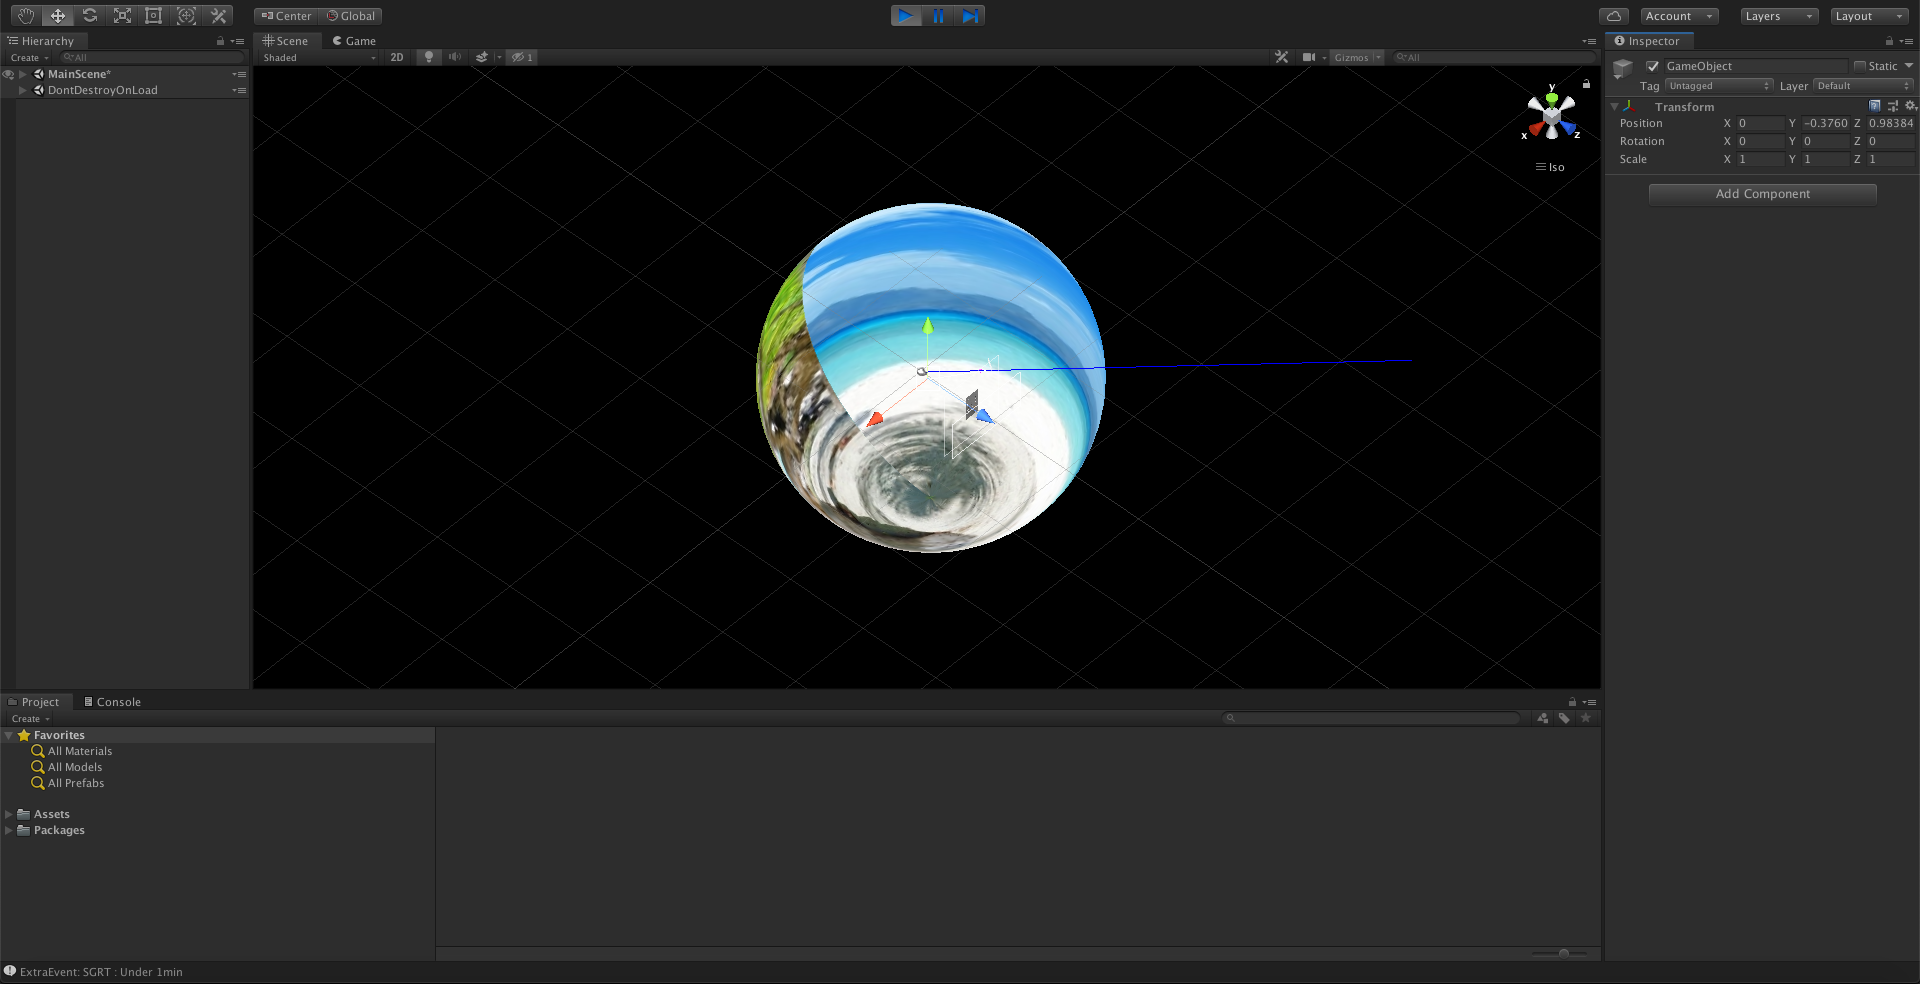
\includegraphics[scale=0.22]{images/Video_Sphere.png}}
    \caption{A video running in a sphere surface}
    \label{video-360}
\end{figure*}

Performance is a critical non-functional feature in VR video players because any frame drop is noticed by the user, causing nausea and discomfort. Some studies measure the experience in VR video players such as \cite{yao2019towards}, where the author proposes a model to build a good experience for video players.

\section{Architecture} \label{architecture}

% TODO: Describe how such components are connected
% TODO: Describe how non-functional requirements can be met with this architecture


In the search for an optimized way to use a video player in mobile virtual reality platforms, the architecture is divided in two main layers:

\begin{enumerate}
    \item Platform layer: native implementation to handle I/O operations and file system.
    \item Rendering layer: use of a render framework to make the 3D virtual universe visible.
\end{enumerate}

This architecture (Figure \ref{fig-video-player-arch}) aims to (1) organize the communication between all modules present in the layers; (2) organize the code to be used by different render engines or different native players; and (3) provide good performance in all media codecs and texture renders.

The platform layer is responsible for media consumption, file system, allocation, and memory management. Some multimedia applications need not only to render digital media but also allow the user to interact with this player.

\begin{figure*}[h]
    \centering
    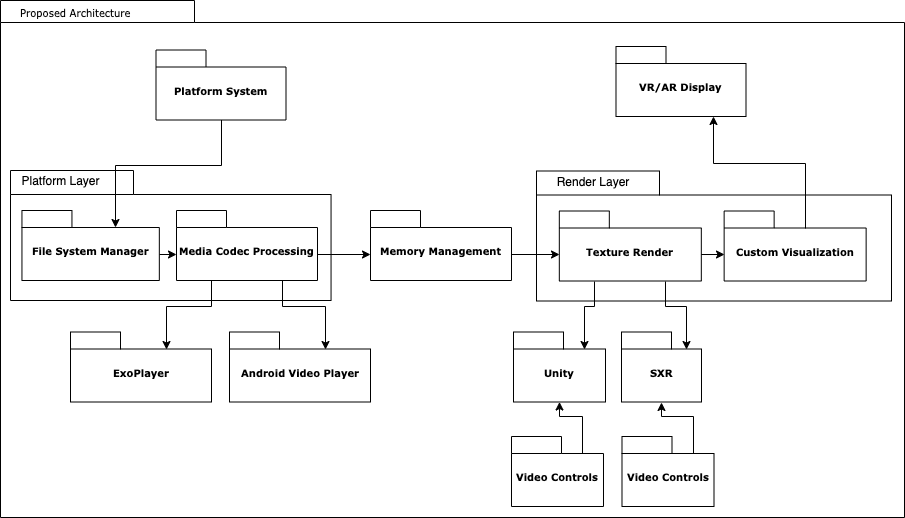
\includegraphics[width=\textwidth]{images/ProposedArch.png}
    \caption{Proposed architecture for Video Player}
    \label{fig-video-player-arch}
\end{figure*}

\subsection{Rendering layer}
% Afonso
The rendering layer is responsible for getting the digital media content and make it visible on the display once it is processed by the codec/native player and provided to the memory buffer. Therefore, it is necessary to use a rendering engine that can receive the memory buffer and render the content on a surface.

Both rendering engines (Unity and SXR) used in this work are capable of applying this rendering process in a good and efficient way. Both engines can use low level graphics API, such as Vulkan \cite{VULKAN} and OpenGL ES \cite{OPENGLES}, which provides a flexible and powerful interface between software and graphics acceleration hardware for embedded devices.

Rendering in textures is not so discussed and is one of the least documented parts of literature. The use of textures allows the update and continuous rendering of dynamic components such as websites and videos. For static objects, the best approach is to work with bitmap, for example.

In this context, it is known that applications that use the graphics API commonly create several textures during its execution time. In this case, the higher the resolution textures, the better the graphics are. But with the increased resolution, more memory is required for management, and more time is spent during texture loading. One way to improve the application's performance, battery consumption, device heating and even decrease the size of the generated application binary is to make use of hardware accelerated formats.

\subsection{Platform layer}
% Atacilio
The Platform layer is composed of two parts that provide the baseline for the Video Player Architecture for Virtual Reality on Mobile Devices. They are:

\begin{itemize}
    \item \textit{File System Manager}: in charge of the media file usage and organization;
    \item \textit{Media Codec Processing}: process media files that are loaded for Render Layer.
\end{itemize}

These parts will be explored in the following sections.

\subsubsection{File System Manager}

The main objective of the File System Manager is to provide a centralized and organized data layer composed of multimedia files. This layer must provide all files transparently so that the player has an unique way of working with any type of media.

\begin{figure*}[h!]
    \centerline{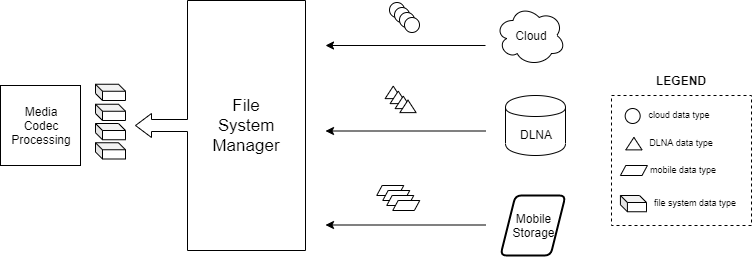
\includegraphics[scale=0.5]{images/file_system2.png}}
    \caption{File System Manager environment}
    \label{fig-file-system}
\end{figure*}

A robust file system manager must implement an interface to output data in the order the video player handles it, even if it comes from different sources (figure \ref{fig-file-system}). In this case,
the file system manager needs to parse all data received from any cloud server, from its own mobile storage or even from a DLNA (\textit{Digital Living Network Alliance}) server and use the defined interface to provide a unique data type that will be processed by the Media Codec.

\subsubsection{Media Codec Processing}

Any multimedia application that plays video must not only render digital media but also needs to provide the status of the currently playing file and controls that enable interaction. These requirements are important, considering they define the possibilities each media player provides for the end-user.

In the Android platform, it is possible to create a media player using one of the following technologies:

\begin{itemize}
    \item \textit{Media Player class \cite{MediaPlayer}}: provides basic controls to reproduce audio and video files;
    \item \textit{Exo Player library}: the ExoPlayer \cite{Exo}\cite{ExoPlayerHello} library defines standards for audio and video reproduction.
 It was built using the MediaCodec API with features such as DASH
 (\textit{Dynamic Adaptive Streaming over HTTP}) and HLS (\textit{HTTP Live Streaming}), which are not available in the MediaPlayer class.
\end{itemize}

\begin{figure*}[h!]
    \centerline{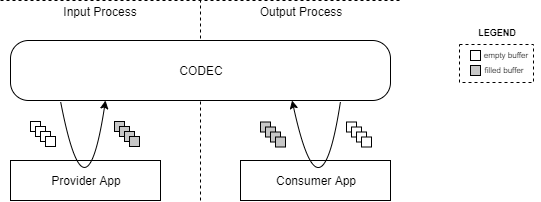
\includegraphics[scale=0.5]{images/codec.png}}
    \caption{Codec process}
    \label{fig-codec}
\end{figure*}

The MediaCodec class offers several possibilities for ExoPlayer by giving access to media codecs at a
low level of implementation. This is possible because codecs convert input data
into output data through multiple I/O buffers processed asynchronously (see figure \ref{fig-codec}).

MediaCodec has the following types of data \cite{MediaCodec}: compressed, raw audio, and raw video. Any of these types can be processed using objects of the ByteBuffer class.

The codec performance is improved when Surface is used for raw video data. This is due to the use of native buffers where it is not necessary to map or copy data for ByteBuffers objects. It is worth mentioning that it is impossible to access raw data when using a Surface. In this case, an object of the ImageReader class is necessary to obtain video frames.

The mimetype of a file defines the compressed data for the input and output buffers. For videos, it is usually just a single frame of compressed video. Regarding video buffers in ByteBuffer mode, they are defined according to the color format that can be \textit{native raw video format}, \textit{flexible YUV buffers} or \textit{others} - generally supported by the ByteBuffer mode through specific format.

As presented on \cite{MediaCodec}, every codec has states that map actions during its life cycle. They can assume the \textit{Stopped}, \textit{Executing} and \textit{Released} states. The Stopped state maps a set of other sub-states that are \textit{Uninitialized}, \textit{Configured} and \textit{Error}. The Executing state builds on other sub-states that are \texit{Flushed}, \textit{Running} and \texit{End-of-Stream}. It's important to know its behavior in order to plan how codec will be used in way that it does not impact other applications.


\subsection{Experiments and Results} \label{experiments}

The experiments were made using three different applications: VR Gallery, SXR Video player, and a demo app. The first application is a fully-featured Unity application supporting many other parallel features besides the video player; the second one is a video player application on the SXR platform, and the last one is a Unity application that implements the architecture presented in this paper.

The graphs below shows the FPS registered in the VR Gallery application.

\begin{figure}[h]
    \centering
    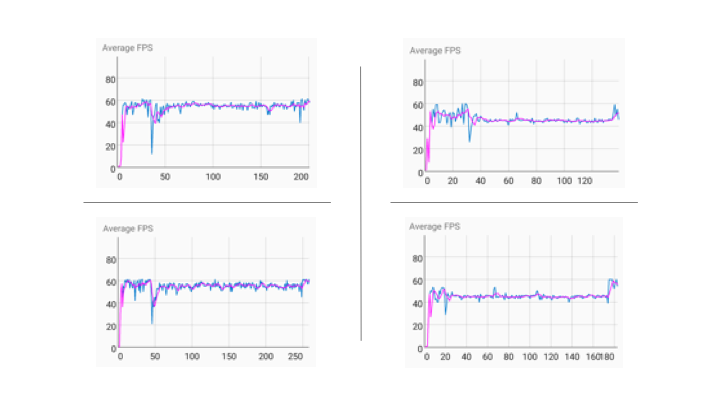
\includegraphics[width=\textwidth, height=6cm]{images/Gallery.png}
    \caption{FPS in VR Gallery}
    \label{gallery-graph}
\end{figure}

According to figure \ref{gallery-graph} and figure \ref{SXR-graph}, the SXR framework maintains 60 FPS in all test cases. However, the initial experiments have shown that the video player of the VR Gallery (application developed in Unity) does not perform well. While Samsung Galaxy S8 Gallery has an fps variation between 55 and 60 FPS, in Samsung Galaxy S6, it stays between 40 and 50 FPS. The reason for these results is the heavy environment VR Gallery has, which is not seen in the other applications.

Even with the mentioned remarks, the user experience was not affected in any of the tests, the video player performed well. The user cannot perceive the difference between both applications and the frame-rate difference is unnoticeable.

The graph below shows the FPS registered by SXR application:

\begin{figure}[h]
    \centering
    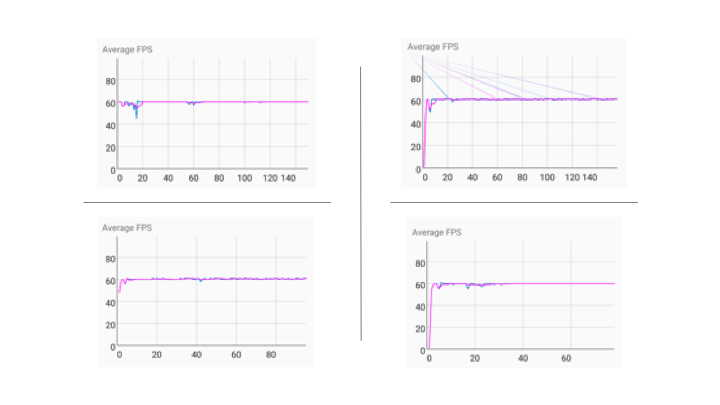
\includegraphics[width=\textwidth]{images/SXR.png}
    \caption{FPS on SXR}
    \label{SXR-graph}
\end{figure}

The difference between both applications is visible. The SXR application has better results, considering its FPS count is around 60 with some small variations. Even though this is a good result, a better behavior can be observed in the last application where the FPS only varies during the application loading and is stable during video execution.

\begin{figure}
    \centering
    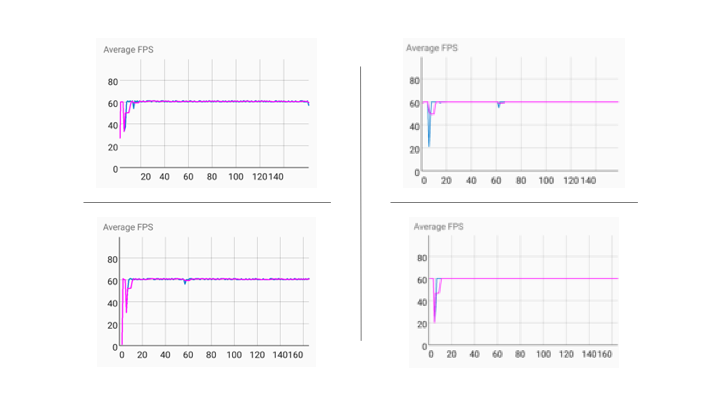
\includegraphics[width=\textwidth, height=6cm]{images/SeparetedApp.png}
    \caption{FPS in the isolated application.}
    \label{app-graph}
\end{figure}

\section{Conclusion} \label{conclusion}
According to the tests, the VR Gallery video player does not have good performance when compared to SXR, however the difference between then can be explained by the fact that the VR Gallery is a complete and robust application, with providers and 3d effects. Even so, the video player of Gallery gives users a complete experience of a good performance video player in a VR environment.

Besides that the video player implemented in unity, that was presented, shows that the proposed architecture delivers a 60 FPS application, without frame drops and lagging, and proved to be very stable even in a full 3d environment application.
%
% ---- Bibliography ----
%
% BibTeX users should specify bibliography style 'splncs04'.
% References will then be sorted and formatted in the correct style.
%
\bibliographystyle{splncs04}
\bibliography{vrvideoplayerarch}

\end{document}
